\documentclass{standalone}
%\usepackage{siunitx}
\usepackage{graphicx}
\usepackage{tikz}
\usetikzlibrary{shapes.geometric, arrows}

\newcommand{\BoxWidth}{1.8cm}%
\tikzset{
    point/.style     = {coordinate},
    arrow/.style     = {thick, ->, >=stealth'},
    to/.style        = {->,>=stealth', shorten >=1pt, semithick, font=\footnotesize, draw=green},
    line/.style      = {line width=0.4mm, draw=blue},
    darrow/.style     = { <->, line width=0.4mm, draw=blue},
    decision/.style  = {draw, diamond, minimum width=\BoxWidth, minimum height=1cm, text centered, aspect=2, font=\footnotesize},
    process/.style   = {draw, rectangle, minimum width=\BoxWidth, minimum height=1cm, text centered, text width=\BoxWidth, font=\footnotesize},
    startstop/.style = {draw, rectangle, rounded corners, minimum width=\BoxWidth, minimum height=1cm,text centered, text width=\BoxWidth, font=\footnotesize},
    box/.style       = {draw, rectangle, minimum height = 1cm, minimum width = \BoxWidth, text centered, text width=\BoxWidth, ultra thin, draw=orange, fill=orange!30, font=\footnotesize},
    smallBox/.style       = {draw, rectangle, minimum height = 0.5cm, minimum width = 0.5cm, text centered, ultra thin, draw=black, fill=green!30, font=\small}
}

\pgfmathsetmacro{\ex}{0.85}
\pgfmathsetmacro{\ey}{0.60}

\begin{document}
\begin{tikzpicture}
	\node[anchor=south west,inner sep=0] (image) at (0,0,0) {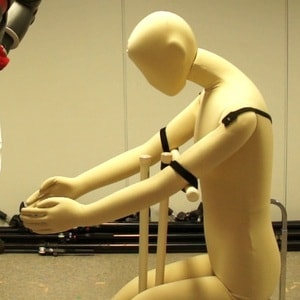
\includegraphics[width=\linewidth]{mannequin}};
	\begin{scope}[x={(image.south east)},y={(image.north west)}]
		\iffalse
		%% Next four lines helps to locate the point needed by forming a grid
		\draw[help lines,xstep=.1,ystep=.1] (0,0) grid (1,1);
		\draw[help lines,xstep=.05,ystep=.05] (0,0) grid (1,1);
		\foreach \x in {0,1,...,9} {\node[anchor=north] at (\x/10,0) {0.\x}; }
		\foreach \y in {0,1,...,9} {\node[anchor=east] at (0,\y/10) {0.\y};}
		\fi
		\begin{scope}[x={(image.south east)},y={(image.north west)}]
			\draw[line] (0.30,0.60) -- (\ex,\ey);
			\draw[line] (0.20,0.25) -- (\ex,\ey);
			\draw[darrow](\ex,\ey) ++(-152:.2) arc (-152:-180:.2) node[xshift=-3cm, yshift=0.5cm, color=blue, font=\large] {Angle of inclination ($\alpha$)} ;
		\end{scope}
	\end{scope}
\end{tikzpicture}
\end{document}